\chapter{Context of the work}
\minitoc
\newpage

\setcounter{secnumdepth}{0}
% ----------------------- Introduction ----------------------- %
\section{Introduction}
This chapter introduces the general context of this report.
We start by presenting the frame of the project as well as the host company.
Then comes the enumeration of the problems which led to the realization of the project.
We wrap it up by defining the methodology we've followed to carry out our work.

\setcounter{secnumdepth}{2}
% ----------------------- General framework of the internship ----------------------- %
\section{General framework of the internship}
This project was carried out within the frame of obtaining a bachelor's degree in Computer Science at the Faculty of Science of Monastir (FSM), Tunisia.
The internship took place over 4 months at Mashroom, an innovative early-stage startup focused on 3D product visualization services. The internship aimed to build a complete, scalable cloud infrastructure from scratch to support the platform's growth and implement modern DevOps and GitOps principles.

% ----------------------- Company overview ----------------------- %
\subsection{Company overview}
This section introduces the host company {\bf Mashroom} as well as the services it offers.

\subsection{About Mashroom}
Mashroom is an innovative platform that enables businesses to easily create, style, and publish beautiful 3D product visuals on demand.
The platform significantly reduces costs and production time compared to traditional photography shoots.
Mashroom combines human design expertise with cutting-edge technology to help companies showcase their products in stunning, hyperrealistic 3D renders.

\begin{figure}[H]
    \centering
    \makebox[\textwidth]{
\includegraphics[width=12cm]{src/assets/logos/mashroom.png}}
    \caption{Logo of Mashroom}
    \label{fig:logo-of-mashroom}
\end{figure}

\subsection{Mashroom's Services}
Mashroom's offering is built around two complementary services: one focused on producing high-quality 3D renders from product photographs, and the other providing a digital environment for managing and reusing this content.

\subsubsection*{\underline{3D Product Visualization}}
Mashroom's core service delivers top-notch 3D product visualization by:
\begin{itemize}
    \item Accepting product photos from clients
    \item Producing hyperrealistic 3D renders that exceed expectations
    \item Delivering professional, publication-ready visual content
    \item Serving diverse industries including furniture, restaurant design, e-commerce, and retail
\end{itemize}

\subsubsection*{\underline{Content Management Platform}}
The platform provides clients with:
\begin{itemize}
    \item Intuitive tools to manage and organize 3D content
    \item Cost-effective alternative to traditional photo production
    \item Faster turnaround times for product visualization
    \item Scalable solutions for businesses of all sizes
\end{itemize}

% ----------------------- Stating the problem ----------------------- %
\section{Stating the problem}
At the start of this internship, the company's entire software platform was running on a single virtual server rented from a cloud provider---an external company such as Amazon Web Services or Google Cloud that rents on-demand computing infrastructure. The two web interfaces seen by clients, the backend service that powered them, and the database that stored customer data all shared the same machine, with no separation between components and no second instance to fall back on. Releases were equally rudimentary: a developer would log into the server through a remote terminal session, pull the latest code, and restart the affected services by hand.

This setup had been good enough during the earliest stages of development, but as the company prepared to open the service to real customers, three limitations became impossible to ignore. The platform could not grow with demand, since a single machine has fixed memory and computing power: traffic spikes degraded performance for everyone, while idle periods cost the same fixed price. The release process offered no flexibility either---there was no way to apply changes automatically, no safety net to undo a faulty release, and no separate environment in which to test a change before exposing it to real users. Finally, reliability was effectively non-existent: the failure of that one machine would take down the entire platform at once, customer data included.

Taken together, these limitations made it clear that incremental fixes would not be enough. The platform needed to be rebuilt on a different foundation---one capable of growing with demand, recovering from failure on its own, and absorbing the steady stream of changes that any real product receives. Defining and building that foundation became the core mission of this internship.

% ----------------------- Assessment of the case ----------------------- %
\section{Assessment of the case}
Before designing a new infrastructure, we must understand precisely what the existing one fails to deliver, and whether the broader industry has already solved problems of this kind. The following subsections review the weaknesses of the current setup, survey the dominant paradigms used to host modern web platforms, and converge on the architectural direction adopted for the rest of this work.

\subsection{Criticizing the current state}
The deficiencies that motivate the rest of this work fall into five distinct categories, each of which the new architecture will need to address explicitly.

\begin{itemize}
    \item \textbf{Single point of failure:} every part of the platform---both web interfaces, the backend service, and the database---ran on the same machine. Any hardware failure, network issue, or misconfiguration would take the entire service offline at once, with no automatic failover in place.

    \item \textbf{No scalability:} the platform could not be made to serve more users without manual intervention. Increasing capacity meant provisioning a new server by hand and reconfiguring the application to run on it---a process far too slow to react to real-time fluctuations in demand.

    \item \textbf{Manual deployments:} each release was carried out step by step by a developer connected to the server, who pulled the new code, installed its dependencies, and restarted the running services in turn. The process was slow, inconsistent, error-prone, and offered no rollback mechanism if the release turned out to be faulty.

    \item \textbf{No environment separation:} there was no dedicated environment in which to try a change before exposing it to real users. Every modification was applied directly to the live service, so any bug introduced during development was felt immediately by customers.

    \item \textbf{Unreproducible infrastructure:} the server had been configured by hand over many months, and no record was kept of the exact steps that had been taken. Rebuilding the same environment on a fresh machine would have required reconstructing the configuration from memory, piece by piece.
\end{itemize}

Each of these categories becomes a non-negotiable requirement for the architecture proposed in the remainder of this chapter.

\subsection{Study of existing solutions}
The requirements identified above mirror challenges that many young technology companies have faced over the past decade, and the industry has converged on a small number of recurring paradigms for hosting modern web platforms. Reviewing these paradigms---and the specific reasons each one falls short of the constraints listed in the previous subsection---clarifies the architectural direction that the rest of this work will pursue.

\subsubsection*{\underline{Function-as-a-Service execution}}
A first paradigm runs application logic as short-lived, event-triggered functions that an external runtime executes on demand---AWS Lambda is the canonical example, with Google's Cloud Functions and Microsoft's Azure Functions playing the same role on competing clouds. The model is attractive for sporadic, stateless workloads, but it cannot serve a platform like Mashroom's: the 3D rendering operations at the heart of the product run for tens of seconds and sometimes several minutes, well beyond the execution-time limits these runtimes enforce.

\subsubsection*{\underline{Fully managed container services}}
A second paradigm relies on third-party services that accept a packaged, runnable application and operate it without exposing the underlying scheduling layer to the user. Heroku popularised this approach in the early 2010s, with more recent equivalents---Google Cloud Run, AWS App Runner, Render, Fly.io---occupying the same space. The convenience comes at a price: each service exposes a proprietary deployment description that does not translate to others, creating strong dependency on a single provider. Patterns this project depends on heavily---declarative continuous delivery, environment-specific configuration overlays, fine-grained autoscaling---are either unsupported or require workarounds that defeat the simplicity these services are sold on.

\subsubsection*{\underline{Managed container orchestration}}
A third paradigm runs the application on a cluster---a coordinated group of machines whose internal scheduling is handled by a piece of software called an orchestrator---operated as a service by the cloud provider. Kubernetes has overwhelmingly won this space, and every major provider now offers it as a managed service---Amazon's EKS, Google's GKE, Microsoft's AKS. This removes the burden of operating the orchestration layer itself while keeping the cluster portable across providers. The paradigm only solves part of the problem, however: the resources around the cluster (networks, databases, secret stores) are usually configured by hand through a web console, with no audit trail; changes to the cluster are typically applied from a developer's machine, with no automated rollback; and separating testing from production demands either two physically separate clusters or an explicit overlay strategy. Managed orchestration is therefore best understood as a strong foundation, not a complete answer.

\subsubsection*{\underline{Synthesis}}
No single paradigm meets all five requirements at a cost the company can afford, but the third comes closest. The architecture proposed here builds on managed orchestration and adds two further layers: one defining every supporting resource declaratively in version-controlled files, and one delivering application changes to the cluster automatically and reversibly. This combination has become the standard pattern at organisations facing the same constraints; the next subsection describes how it was instantiated for Mashroom.

\subsection{Proposed solution}
The architecture proposed for Mashroom's platform builds on the layered pattern described above. Each layer is instantiated to fit the company's constraints; the specific tools chosen at each layer are surveyed and justified in the next chapter.

\subsubsection*{\underline{From a single machine to a managed cluster}}
The application is lifted off its single host onto a managed cluster. Each of the two web interfaces and the backend service is packaged so that it can run on any machine in the cluster. The orchestrator schedules these applications across the cluster, restarts them on failure, adds copies as load grows, and rolls out new versions one at a time, so the platform never goes fully offline during an update. A single cluster serves both production and a dedicated pre-production environment, kept apart by the cluster's own isolation mechanism rather than by duplicated infrastructure.

\subsubsection*{\underline{Reproducible cloud infrastructure}}
Around the cluster sits a constellation of supporting resources: the network in which it lives, the database that stores customer data, the object storage that holds rendered assets, the load balancer that routes incoming traffic, and the secret store that keeps credentials. Each of these is described in declarative configuration files held in a version-controlled directory rather than configured by hand through the cloud provider's web console. This \emph{Infrastructure-as-Code} layer makes the setup auditable and reproducible: every modification is recorded alongside the source code, reviewable before it takes effect.
\subsubsection*{\underline{Automated and reversible delivery}}
The third layer governs how changes reach the cluster. When a developer adds new code, an automated \emph{pipeline} (a sequence of steps triggered by every change) builds, tests, and packages the application. Rather than pushing the new build to the cluster directly, the pipeline updates a set of declarative configuration files describing what the cluster should look like and saves those updates to a version-controlled directory. A separate piece of software watches that directory and reconciles the cluster against it: whenever the files differ from what is actually running, it applies the difference. This indirection---known as \emph{GitOps}---makes deployments fully automated yet fully reversible: undoing a faulty change is no more than reverting the corresponding files. Differences between production and pre-production are handled by an \emph{overlay} mechanism that keeps a common base shared between the two and lets each environment override only what is strictly necessary. Before any change reaches the cloud, the same files are first applied to a local cluster running on the developer's machine, which catches configuration mistakes, broken service connectivity, or faulty overrides without cloud cost or risk to the live service.

\newpage

% ----------------------- Development Methodology ----------------------- %
\section{Development Methodology}

Delivering this project within the four-month internship timeframe required a structured operational approach. This section outlines the methodology used to track, manage, and execute the infrastructure and automation tasks.
\subsection{Adopting Kanban for DevOps Automation}

Kanban is exceptionally well-suited for infrastructure automation due to its inherent flexibility and continuous workflow model [1]. This adaptability provides exactly what is needed in DevOps environments, where technical tasks are often unpredictable and require dynamic reprioritization based on system dependencies or sudden blockers. DevOps itself is a methodology that bridges software development and IT operations to streamline, manage, and automate cloud infrastructure [2]. By managing our work through a visual Kanban board---tracking tasks smoothly from \textit{To Do} through \textit{Done}---we maintained a steady operational flow without being constrained by rigid planning cycles.

\begin{figure}[H]
    \centering
    \makebox[\textwidth]{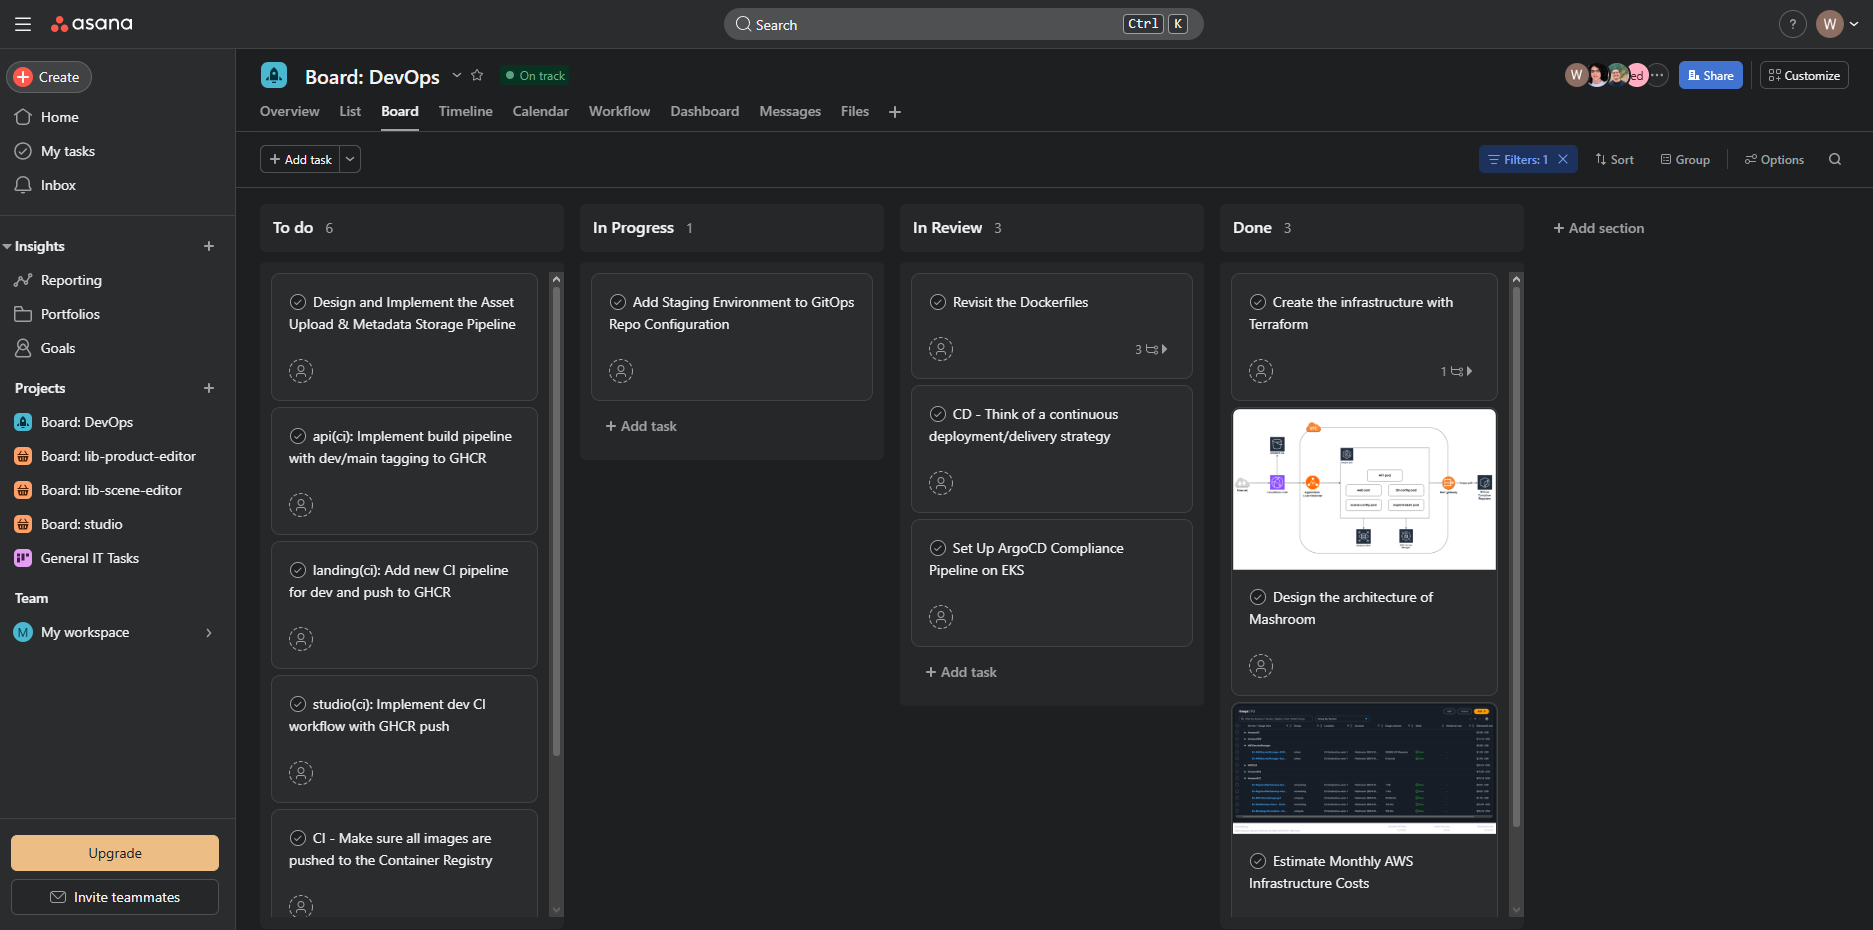
\includegraphics[width=\linewidth]{src/assets/screenshots/asana.png}}
    \caption{Project Kanban board on Asana}
    \label{fig:asana-kanban-board}
\end{figure}


\setcounter{secnumdepth}{0} % Set the section counter to 0 so next section is not counted in toc
% ----------------------- Conclusion ----------------------- %
\section{Conclusion}

In this chapter, we presented not only the host organization but also the general context of the project and the critical need for a modern cloud architecture. We then evaluated the limitations of the existing single-server setup and discussed the possible development methodologies to manage this transition. Lastly, we selected the most ideal choice for our DevOps workflow, which is Kanban.